% simple.tex -- a very simple thesis document for demonstrating
%   dalthesis.cls class file
\documentclass[12pt]{dalthesis}

\usepackage{graphicx}	% Including figure files
\usepackage{amsmath}	% Advanced maths commands
\usepackage{amssymb}	% Extra maths symbols


\begin{document}

\title{Predicting Canadian Consumer Food Prices with Python}
\author{Patrick Walter}

% The following degrees are included in the current dalthesis.cls
% class file:
\bcshon  % options are \mcs, \macs, \mec, \mhi, \phd, and \bcshon

% If you degree is not included, you can set several options manually.
% The following example shows the parameters for the \mcs degree.
% However, if you need to set these parameters manually, please check
% the correct names with the Faculty of Graduate Studies, and let the
% maintainer of this class file know (Vlado Keselj, vlado@cs.dal.ca).
% MCS Example:

\degree{Bachelor of Computer Science}
\degreeinitial{BCS}
\faculty{Computer Science}
\dept{Faculty of Computer Science}

% Month and Year of Defence
\defencemonth{July}\defenceyear{2018}

% This sample thesis contains no tables nor figures, so there is no
% need to include lists of tables and figures in the front matter:
\nolistoftables
\nolistoffigures


\dedicate{This thesis is dedicated to my parents. For their endless love, support, and encouragement.}



\frontmatter

\begin{abstract}
Based on the work done for Canada Food Price Report 2017, this research attempts to use historic econometric and financial data to predict the price of individual and aggregate food products contained in the basket of the Canadian Consumer Price Index using Python Scikit Learn linear regression models coupled with mutual information feature selection. Models were trained and evaluated for their predictions of the food price portion of Canadian Consumer Price Index basket for a five-year period between 2012 to 2016. Further research was then done to train models to predict each of twenty-two individual targets of individual and aggregate consumer products from the Canadian Consumer Price Index basket for the years of 2016 and 2017. Lastly ensemble methods were used to train 17 linear regression models and aggregate their predictions in an attempt to make a more stable model with more generalized predictions which were tested on the years 2016 and 2017.
\end{abstract}

\begin{acknowledgements}
Thanks to my advisor Dr. Vlado Keselj.
\end{acknowledgements}

\mainmatter

\chapter{Introduction}

\section{Consumer Price Index}

The Canadian Consumer Price Index is an indicator of the changes in prices experienced by Canadians obtained by comparing the rising or falling cost of a fixed basket of good and services purchased by Canadians. A fixed basket means that it contains goods and services of the same quantity and quality and therefore the changes in cost are a true reflection of the pure price changes \cite{statscan}.  The Consumer Price Index is released monthly for each province and national averages are computed. The Consumer Price Index is divided into eight categories which include: food, shelter, household operations and furnishings, clothing and footwear, transportation, health and personal care, recreation, education and reading, and alcoholic beverages and tobacco products. There are also three special aggregates which include: all items excluding food, all items excluding energy, and energy. These categories are then divided into subcategories which are then divided into even more refined values, some of which represent specific individual food products such as different meats, seafood, and dairy products. \\

The main purpose of the Canadian Consumer Price Index is to be an indicator of the changes in the level of consumer prices which reflects the rate of inflation. Since inflation is a direct factor of purchasing power the CPI is useful to all Canadians who can compare the changes in their own personal income with those shown by the CPI to assess their personal financial situation. Most governments and economists believe that a small positive value for inflation is optimal for allowing producers to increase the quality of products and services \cite{jay}. 

\section{Canada Food Price Report}

Beginning in 2010, The Canada Food Price Report has set out to be a tool used to forecast Canadian food prices and focus on the factors that will be affecting the future of consumer food prices over the following one-year period. The report began at University of Guelph by Dr. Sylvain Charlebois and Dr. Francis Tapon and is now a publication by Dalhousie University. The report combines information from several food-related reports and data to identify the key fundamental drivers that will impact food prices for the year ahead. These drivers are categorized into macro, sectorial, and domestic \cite{foodreport17}. Beginning in 2017 the report has started to employ machine learning models to be used to support the opinions of a panel of experts. The models used many financial features with reliable data from 1999 to 2016 as the independent variables. \cite{foodreport17}



\section{Research Objectives}
The main objective of this research was to predict the aggregate food price of the CPI using a linear regression model implemented in python using Scikit Learn. This lead to three separate experiments each with its own research objectives. The first was to implement linear regression models that used the acquired dataset from the 2017 report to predict the target variable of average food price from the CPI basket. This lead to subsequent research and experiments on how to apply feature selection using mutual information to reduce the dimensionality of the model to 
make more accurate predictions. To test this, individual models were constructed to predict the monthly average food price for the twelve-month period of each year from 2012 to 2016. The target values 
for these predictions were sourced from Statistics Canada and the attributes dataset was a subset of the 
dataset produced by Jay Harris for the research done for the Canada Food Price Report 2017 and 
subsequent report in 2018. The results from this experiment showed which years in that time period were able to be predicted with greatest accuracy. \\

The second objective of this research was to implement linear regression models coupled with the above feature selection methods and dataset to predict other targets in the CPI basket. This research attempted to predict twenty-one other primarily food 
related subcategories of the CPI basket for the years of 2016 and 2017. In this experiment the goal was to identify the specific subcategories of the average food price and other products that were most difficult to predict accurately with the same dataset. This work created 22 independent models for predicting each of the targets which were tested for their accuracy on the test years of 2016 and 2017. \\

The third objective of this research was to implement a ensemble of linear regression models that would be used together as an aggregated system of models to better predict the average food price of the CPI for the year 2016. The earlier models created to predict the average food price for the year 2016 were used as a baseline to compare against ensemble methods implemented by used a modified version of the bootstrap aggregating algorithm. This work created a set of models that employed different methods of aggregating the outputs of  individual models to create an ensemble. This included an averaging, a weighted averaging, and an inflation adjusted averaging method. \\

\chapter{Related Work}
\section{Related Work}

A 2017 thesis written by Jay Harris titled A Machine Learning Approach to Forecasting Consumer Food Prices was a key related work in this project. The objective of that research was to test methods of predicting food prices for Canadian Consumers to determine the best method of forecasting. The paper compared baseline approaches commonly used in financial and econometric forecasting against machine learning techniques such as linear regression. This work illustrated the accuracy of these machine learning techniques when applied to consumer food price forecasting. \cite{jay} The machine learning approaches of that research were implemented in WEKA, a data mining and machine learning software suite with a graphical user interface. While WEKA is a good tool for testing machine learning strategies, more sophisticated tools can be used to develop more complete systems. \cite{jay} This motivated the use of a programming language such as python to implement similar machine learning approaches applied to similar research objectives. \\

In 2017, the Canada Food Price Report employed a machine learning model to supplement the panel of domain experts’ advice \cite{foodreport17}. It leveraged a combination of different machine learning methodologies, including linear regression and support vector machines, to forecast components of the Canadian Consumer Price Index. This was built on a research thesis done by Jabez (Jay) Harris which compared different machine learning algorithms ability to make econometric models to forecast food group categories listed in the Canada Consumer Price Index against benchmark models commonly used in financial and econometric forecasting \cite{jay}. In the report there were over twenty independent variables identified as potential inputs to the machine learning models and of these only ones that were highly correlated with a food categories price were used. These independent variables included household income, immigrant income, income distribution, international aid, population, unemployment, commodity futures, fuel prices, crude oil prices, energy indexes, CDN exchange rate, U.S. overnight lending rates, global agricultural production, global rainfall, commodity prices and global temperatures. \cite{foodreport17}. The input variables used in this report and related thesis work was used as the dataset for this research.







\chapter{Research Methodology}

\section{Dataset}
The dataset of this research was adopted from the work done by Jay Harris of Dalhousie University in a thesis titled A Machine Learning Approach to Forecasting Consumer Food Prices. The targets dataset included twenty-two different targets of which seventeen were food related, all from the CPI categories and special aggregates sourced from Statistics Canada. Some targets are specific food products such as eggs and coffee, while other are aggregates such as food from restaurants and food from stores. This historical dataset begins January 1985 and has monthly records until August 2017. During this research this was updated to include records up until the most recently released month which, at time of writing, was April 2018.  The attributes dataset contained 280 independent features. This was significantly less than the dataset used in the previous thesis which consisted of 476 features before feature selection. The starting record for this dataset was also January 1985, however not all features have values in the early years. The dataset has 391 records which conclude at July of 2017. However, not all features had values for records near the end date. \\

In the Canada Food Price Report 2017 the historical data was capped at January of 1999. This decision was two-fold. Firstly, as mentioned some of the features do not have records for earlier years, and those that do may not be reliable. Secondly in 1997 the Canada Harmonized Sales Tax was implemented which had an effect of consumer prices in Atlantic provinces \cite{jay}. In this research the entire historic data set was used for feature selection but like the Food Report only records after January 1999 were used in training the models.  

\section{Machine Learning in Python}
Python was chosen for this research because it is a full-fledged language with robust machine learning and data mining libraries. Scikit Learn is a machine learning library for the Python programming language which includes implementations of popular machine learning algorithms including regression. Scikit Learn was used for it’s machine learning and modeling capabilities for this research. Other libraries used in this research include Pandas and Matplotlib. Pandas is an open source data structures and data analysis library used for data wrangling and structuring \cite{pandas}. Matplotlib is a 2D plotting library used for data visualization \cite{matplot}. 


\section{Data Preprocessing}
The original dataset contained all features and targets together in a comma-separated values formatted file. This was divided into two comma-separated values files, one for the features and one for the targets. The timestamps feature from the original dataset was copied to both files. Panda’s dataframes were used to structure the datasets for modeling. A dataframe is two-dimensional tabular data structure with labeled axes, which allowed for the time series of each feature and target to be selected by name.\cite{pandas} The two comma-separated values files containing the attributes and targets datasets were imported into two dataframes respectively. These dataframes contained 391 records beginning at January 1985. Reduced versions of these dataframes were constructed beginning at January 1999. The complete dataframes were to be used by feature selection, while the reduced dataframes,  and further partitions, were to be used for training the linear regression models.  As mentioned, some of the records in the attributes dataset had missing values for some of there features in the latest years. To deal with missing values in records, any feature that had missing values after January 1999 was removed. This was a simple solution but only affected a few features. Other solutions, such as predicting future values using linear regression or averaging, were discussed for the future experiments.  \\

Further data preprocessing was done using these four dataframes for each of the three main experiments conducted in this research project. The first was to divide the attributes dataframes into test and train sets for different years. The second was to divide the targets dataframe into individual time series for each of the targets. The third was similar to the first only done further back into the time series. These processes will be described in detail in the experiment section of this paper. 

\section{Linear Regression}

Linear regression is a method of predicting a target value, which is expected to be a linear combination of weighted input variables; where the weights are represented by coefficients and an intercept. The ordinary least squares implementation of linear regression creates a linear model with a vector of weights, or coefficients, that minimizes the residual sum of squares between targets in the dataset and predicted targets.\cite{sklearn} The ordinary least squares implementation from the Scikit Learn library was used for this research. Linear regression was an obvious choice for this work as the goal of most of this research is predicting continuous values that are expected to be a linear combination of the features in the dataset.

\section{Feature Selection}

Feature selection is an important step in creating stable and generalized predictive models. It allows a model to only include the features which are believed to be most important factor effecting the target value. This helps to remove as much redundant, irrelevant, and possibly misleading data as possible.\cite{jay}  Feature selection requires a heuristic scoring function to evaluate the importance of a feature in its usefulness in the model to predict the target values. Some scoring only look at the level of variance to remove feature with little variance which gives a bias to features with higher variance. Other methods focus on the correlation between each individual feature and the target variable. One such scoring function to evaluate the importance of a feature is mutual information between the feature and the target variable. \\

An implementation of mutual information feature selection was used to select a set number of features from the total set of all features in the dataset. Mutual information measures the dependency of two variables and gives a non-negative value. Scikit Learn has an implementation of mutual information for feature selection for both regression and classification. The regression version of the mutual information feature selection uses an estimate of entropy for continuous target variable (Scikit Learn, 2017). This implementation uses a method of entropy estimation based on work by Alexander Kraskov, Harald Stögbauer, and Peter Grassberger which uses entropy estimates from k-nearest neighbor distances to estimate mutual information \cite{mutualinfo} . Unlike other estimates of independence or correlation between variables, mutual information also picks up dependences that are not seen in linear correlation coefficients because they are not shown in covariance \cite{sklearn}.  

\section{K Best}

In this project, mutual information feature selection was used as a scoring function. Each of the features was given a score based on its mutual information score with the target variable. These scores are then used by the SelectKBest feature selection function. This takes the top k scoring features, where k is an integer value between one and the total number of features in the dataset to select from. The value of k is an important hyper-parameter that has a strong effect on the models created. Finding the optimal value for k was part of the experimentation of this project. The scoring can be based on different methods of evaluating correlation and in this research mutual information was used.

\section{Ensembles and Bootstrap Aggregating}
Ensemble methods in machine learning are algorithms that build a set of classifier or regression models using samples of training data and then classify or predict targets for new unseen data by taking votes from the classifier models or an average of the regression models. The purpose of using ensemble methods is to generate more stable and generalized models that will have greater predictive power than individual models. A popular ensemble method is bootstrap aggregating or bagging.\cite{ensemble} \\

Bagging is a method of ensemble which uses random partitions of the training data to train multiple models. Normally each model is of the same type and the training data for each model is generated by randomly sampling from the training set with replacement. To use bagging with a linear regression model, multiple linear regression models are trained on the individual random samples or partitions of the training data. Then all these models are used to make predictions on the same testing data. The predicted output values of each of the models is then aggregated. The outcome of the system of models is then generated by taking the average of all predicted values produced by the individual models \cite{bagging}. Various methods of bootstrap aggregating were used in this research to attempt to create better predictive models. 





\chapter{Experimentation}

\section{Predicting the Average Food Price for a Five-Year Period}


The first objective of the experimentation in this research project was to predict a twelve-month period of an aggregate target labeled Food17, which includes all food products captured in the Canada Consumer Price Index, for each year in a five-year period between 2012 and 2016. These years were selected as they were the last five years with complete twelve-month records in the attributes dataframe.\\ 

To achieve this objective, the attributes dataframe was divided into a testing set and training set for each of the five years in the five-year period. The training and testing sets were constructed for each year as follows. The training set contained the reduced historical data, beginning at January 1999, up until December of the year before the target year and the testing set contained the twelve records of the target year. For example, the training set for the year 2016 was from January 1999 to December 2015, and the training set contained the twelve months from January 2016 to December 2016. This was done for each of the five years to produce ten dataframes, five training sets, and five testing sets. Each pair of training and testing sets were used to train and evaluate the five linear regressions models. \\

Feature selection was conducted using the entire attributes dataframe and the Food17 target dataframe. This used k-best selection based on mutual information scores. Values in the range of 5 to 35 were used for the value of k. For some years, such as 2013 and 2014, values of k less than 10 yielded the best results in terms of mean absolute error and variance scores. For other years, specifically for 2016, a greater number of features were needed to make sufficiently accurate predictions. What was different about the year 2016 was that it was the only year in the five-year period that the food price target had a downward trend. Based on these observations, further work on how to accurate predict irregular years, or crashes, were proposed. Also, further work to create an implementation where the feature selection is done individually for each year using an optimal value for k. \\

Results from this experiment were varied by year. With varying values of k, each model was able to predict the twelve-month period of the average food price target Food17 with mean absolute errors between 0.5 and 3.8. The mean absolute error and variance score for each of the 5 linear regression models for the 5 year period can be seen in Table 3.1 The resulting linear regression models for the five year period using twenty five features can be seen in Figure 3.1. Lastly the linear regression modeled created by the 2012 year was tested for its stability and preditive power on the four subsequent year's training sets. This means that the model that was trained on data records ending December 2011 was tested on four sets of 12 month records for the four subsequent years. The results of this can be seen in Table 3.2. \\


\begin{table}
	\caption{The mean absolute error and variance scores for each of the five linear regression models using the top 7 features selected using mutual information between each feature and the target. }
	\label{tab:5yearerrors}
    \begin{tabular}{ |p{4cm}||p{4cm}|p{4cm}|p{4cm}|  }
       \hline
       \multicolumn{3}{|c|}{5 Year Linear Regression k=7} \\
       \hline
       Year    & Mean Absolute Error    & Variance Score \\
       \hline
       2016    & 2.53    & -1.99\\
       2015    & 3.00    & -9.28\\
       2014    & 0.62    & 0.56\\
       2013    & 0.70    & -3.76\\
       2012    & 0.65    & -0.99\\
       \hline
    \end{tabular}
\end{table}

\begin{table}
	\caption{The mean absolute error and variance scores for the 2012 linear regression model from the last experiment tested on test data for each of the five years in the period. }
	\label{tab:5yearson2012}
    \begin{tabular}{ |p{4cm}||p{4cm}|p{4cm}|p{4cm}|  }
       \hline
       \multicolumn{3}{|c|}{5 Year Linear Regression k=7} \\
       \hline
       Year    & Mean Absolute Error    & Variance Score \\
       \hline
       2016    & 3.21    & -4.02\\
       2015    & 3.02    & -9.39\\
       2014    & 0.65    & 0.55\\
       2013    & 0.65    & -2.06\\
       2012    & 0.65    & -0.99\\
       \hline
    \end{tabular}
\end{table}

\begin{figure}
	% To include a figure from a file named example.*
	% Allowable file formats are eps or ps if compiling using latex
	% or pdf, png, jpg if compiling using pdflatex
	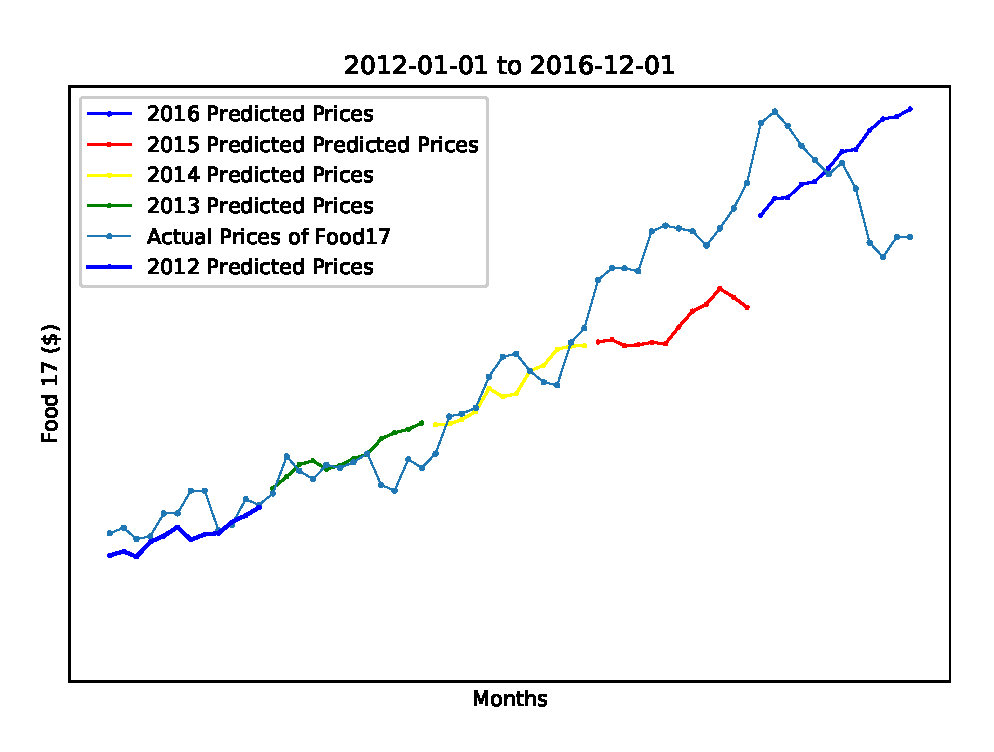
\includegraphics[width=\columnwidth]{5year}
    \caption{The predicted and actual prices for the food portion of the Canadian Consumer Price Index (Food17) for each year in the five year period between 2012 and 2016. The predicted price values for each year are predicted by individual linear regression models trained on data from January 1999 to December of the year prior.}
    \label{fig:5yeargraph}
\end{figure}

\section{Predicting Each Individual Target}
The next experiment was to train models to predict each of the other twenty-one targets included in the targets dataset. The objective of this was to shed light on which products’ prices can be predicted accurately using features selected from the total attributes dataset. In this experiment the process of feature selection was done using mutual information of each of the random variables in the attributes dataframe for each of the twenty-two target variables. \\

This experiment was first preformed for the year of 2017 after the target dataset was expanded using the up-to-date data from Statistics Canada. Unfortunately, the much larger attributes dataset was not able to be updated. The attributes data of the twelve-month period of 2016 was used as the testing data to predict each of the individual targets for the 2017 twelve-month period. This was not ideal for evaluating the model however it was more representative of real world forecasting when a future year is being forecasted based on values from the last year. \\

The targets dataframe was divided into twenty-two one dimensional time series for each of the twenty two targets. These individual targets were then used as the target for individual models. The K-Best feature selection using mutual information scores was again used. This time each experiment had its own feature selection process with the different targets. For each of the targets the mutual information score was computed between that target and each of the attributes in the attributes dataframe. The KBest selector was used again to select the top k scoring features. For this experiment k was set to 10 and was increased to 29 for targets that had poor accuracy. Further research could be conducted to optimize the value of k for each target. \\

A linear regression model was constructed for each of the consumer product targets with the training set constructed using all records between January 1999 and December 2015 using the features selected by the feature selection process. As mentioned before, the testing set was constructed using the records from the twelve months of 2016. Some observations include that many of same features were selected for each of the very different individual and aggregate targets. The aggregate targets were easier to be predict with fewer features and the individual products such as eggs, beef, and vegetables required higher dimensionality to capture their trend. Some targets were able to be predicted accurately using 2016 attributes data, while other had large variance between the predicted values and the actual target values. The mean absolute error and variance scores for each of the targets tested on year 2017 as shown in Table 4.3. The results of the same models tested on the year 2016, a year for which the attributes of that year are included in the training set are seen in Table 4.4. \\


% table for the 2017 targets
\begin{table}
	\caption{The mean absolute error and variance scores for each of the 22 individual targets from the CPI basket for the year 2017. }
	\label{tab:targets2017}
    \begin{tabular}{ |p{5cm}||p{4cm}|p{4cm}|p{4cm}|  }
       \hline
       \multicolumn{3}{|c|}{Individual Category Linear Regression } \\
       \hline
       Category    & Mean Absolute Error    & Variance Score \\
       \hline
       Food 17    & 0.69    & 0.55\\
       restaurants 17    & 3.80    & -11.92\\
       Vegetables    & 5.79    & -0.58\\
       Other    & 1.07    & -1.43\\
       Meat    & 1.07    & -1.43\\
       Dairy products and eggs    &2.56    & -9.70\\
       Bakery    & 3.68    & -6.72\\
       Fruit    & 4.00    & -0.53\\
       All-items    & 1.67    & -4.13\\
       Food purchased from stores    & 1.97    & -1.15\\
       Fresh or frozen beef    & 7.17    & -9.90\\
       Fresh or frozen pork    & 3.60    & -2.39\\
       Fresh or frozen chicken    & 2.19    & -0.35\\
       Dairy products    & 1.99    & -7.39\\
       Eggs    & 7.57    & -3.72\\
       Coffee    & 4.99    & -11.58\\
       Baby foods    & 4.04    & -20.96\\
       Shelter 18    & 2.38    & -16.09\\
       Transportation    & 4.24    & -6.56\\
       Gasoline    & 10.13    & -3.60\\
       Energy 25    & -6.33    & -7.00\\
       Fish seafood    & 5.21    & -3.28\\
       \hline
    \end{tabular}
\end{table}

% table for the 2016 targets

\begin{table}
	\caption{The mean absolute error and variance scores for each of the 22 individual targets from the CPI basket for the year 2016. }
	\label{tab:targets2016}
    \begin{tabular}{ |p{5cm}||p{4cm}|p{4cm}|p{4cm}|  }
       \hline
       \multicolumn{3}{|c|}{Individual Category Linear Regression } \\
       \hline
       Category    & Mean Absolute Error    & Variance Score \\
       \hline
       Food 17    & 2.84    & -2.85\\
       restaurants 17    & 3.61    & -13.43\\
       Vegetables    & 9.56    & -0.59\\
       Other    & 2.64    & -4.09\\
       Meat    & 2.13    & -1.56\\
       Dairy products and eggs    &1.54    & -0.85\\
       Bakery    & 3.11    & -0.96\\
       Fruit    & 7.20    & -1.30\\
       All-items    & 1.48    & -3.63\\
       Food purchased from stores    & 3.31    & -0.85\\
       Fresh or frozen beef    & 6.67    & -1.26\\
       Fresh or frozen pork    & 2.84    & -1.89\\
       Fresh or frozen chicken    & 1.50    & -0.23\\
       Dairy products    & 1.50    & -0.98\\
       Eggs    & 3.48    & -0.31\\
       Coffee    & 3.89    & -2.55\\
       Baby foods    & 4.58    & -17.71\\
       Shelter 18    & 1.95    & -3.55\\
       Transportation    & 2.1    & -0.50\\
       Gasoline    & 11.57    & -1.55\\
       Energy 25    & 8.17    & -2.47\\
       Fish seafood    & 4.71    & -5.63\\
       \hline
    \end{tabular}
\end{table}




%This same experiment was repeated for the year 2016. Results for 2016 were somewhat worst than those of 2017 which was attributed to the downward trend of many of the targets that year. Again, a solution to this problem was to raise the value of k to attempt to capture the downward trend of the year. The results of this experiment for each of the 22 target variables are shown in figure 4.3 Further work on how to better predict years will be conducted and discussed in the further research section. \\

\section{Predicting Average Food Price with Ensemble Methods}



The objective of this part of experimentation of this research was to attempt to apply modified ensemble methods to build a bootstrapped aggregate linear regression model with greater stability and stronger predictive power. What needed to be modified from the normal bootstrap aggregating method was how to sample the training data. In the normal bootstrap aggregating algorithm a random sample of the training data with replacement is taken for each of the individual models that will be aggregated in the system. This creates a set of partitions of the data that are possibly overlapping.  For a time-series dataset like the one used in this research, a random sampling of the data is not suitable. With a time series dataset each exemplar in the total training set are in order and should remain in order. \\

In this research a different method what was applied to sample the data set to create the individual training sets for each of the individual models in the ensemble. The method of sampling was to partition the data in the same way that the data was partitioned to train and test the linear regression models for the five year period in section 3.1. This method of partitioning was extended past five years to 17 years. In total 17 samples of the training data were taken with replacement. The first included January 1999 to December 2016. Each subsequent partition began at January 1999 and ended with December of the year prior to that of the last partition. This created 17 training sets to be used to train 17 unique and separate linear regression models. \\

Another method of sampling or partitioning the data would be to portion the data into 17 portions of 12 months each for the last 17 years of the dataset. This method would be a form of sampling without replacement. This would reduce the bias of the ensemble system towards records from earlier years as these records are duplicated in more of the training data sets than later years. However this method proved ineffective as the size of the training sets being only 12 exemplars made for poor predictive power and great instability. \\

The 17 models were trained using their respective training data sets and then tested on their test year, the corresponding target year of their last year in their training set. The results of this testing varied. Some models were able to be predict their target values with minimal absolute error, but nearly all years had negative variance scores meaning the models did not explain the changes in price well. It is important to note that the poor accuracy of some years may be due to economic activity that took place during that year such as recession and recovery periods. The results of these models can be seen in Table 3.5. The same 17 models were next tested on one year into the future, in other words the year after their last record in their attributes training set. Again this is more real world applicable of forecasting without the corresponding year's data. The results of this can be seen in Figure 3.6. Again the performance based on the mean absolute error was minimal for most years, but the extremely high negative values of variance scores of some years shows the models failing to capture the explain the changes in prices incurred. \\

Next these  17 models were combined to create an ensemble. First each of these models are used on the 2016 testing data to produce 17 outputs of predicted average food prices for the 12 month period of 2016. These predictions are then averaged to complete the ensemble system.  The resulting output of this ensemble was very poor with a mean absolute error of 9.09. The same ensemble was then tested on the year 
2000, the first year of the period. The result of this was good with a mean absolute error of only 0.40, however their is no practical use of this as uses more recent data to predict the past. The next ensemble to test was created the same way but only used the last 10 years instead of 17. The average predictions of these 10 models tested on year 2016 gave a much better result. Results of all of these models can be seen in Table 3.7.\\






\begin{table}
	\caption{The mean absolute error and variance scores for each of the 17 linear regression models using the top 18 features selected using mutual information between each feature and the target. Each model was tested on the corresponding year following the last record in the sample data set for that model.}
	\label{tab:17years}
    \begin{tabular}{ |p{4cm}||p{4cm}|p{4cm}|p{4cm}|  }
       \hline
       \multicolumn{3}{|c|}{17 Linear Regression to be Used in Ensemble Methods } \\
       \hline
       Year    & Mean Absolute Error    & Variance Score \\
       \hline
       2016    & 2.11    & -1.18\\
       2015    & 2.60    & -6.64\\
       2014    & 1.42    & -0.64\\
       2013    & 1.07    & -5.88\\
       2012    & 3.68    & -43.52\\
       2011    & 1.04    & -0.05\\
       2010    & 1.43    & -14.08\\
       2009    & 1.64    & -1.30\\
       2008    & 1.28    & 0.64\\
       2007    & 2.77    & -26.68\\
       2006    & 1.31    & -4.50\\
       2005    & 5.54    & -62.06\\
       2004    & 1.51    & -2.08\\
       2003    & 1.65    & -13.18\\
       2002    & 3.65    & -41.49\\
       2001    & 1.09    & -0.97\\
       2000    & 2.89    & -11.44\\
       \hline
    \end{tabular}
\end{table} 

\begin{figure}
	% To include a figure from a file named example.*
	% Allowable file formats are eps or ps if compiling using latex
	% or pdf, png, jpg if compiling using pdflatex
	\includegraphics[width=\columnwidth]{errorplot}
    \caption{The mean square error of each of the 17 models. Each model was trained on the sample set of the data that ends December of the year before and tested on the 12 month period of the corresponding year following.}
    \label{fig:allyearerror}
\end{figure}


\begin{table}
	\caption{The mean absolute error and variance scores for each of the 17 linear regression models using the top 18 features selected using mutual information between each feature and the target. Each model was tested on the corresponding year following the last record in the sample data set for that model.}
	\label{tab:17years}
    \begin{tabular}{ |p{4cm}||p{4cm}|p{4cm}|p{4cm}|  }
       \hline
       \multicolumn{3}{|c|}{17 Linear Regression to be Used in Ensemble Methods } \\
       \hline
       Year    & Mean Absolute Error    & Variance Score\\
       \hline
       2017    & 1.14    & -1.56\\
       2016    & 2.20    & -1.21\\
       2015    & 0.51    & 0.49\\
       2014    & 1.56    & -2.15\\
       2013    & 1.83    & -17.19\\
       2012    & 1.83    & -11.84\\
       2011    & 2.87    & -3.58\\
       2010    & 4.28    & -122.96\\
       2009    & 3.44    & -41.29\\
       2008    & 1.67    & 0.31\\
       2007    & 2.17    & -18.15\\
       2006    & 4.55    & -54.90\\
       2005    & 0.86    & -0.98\\
       2004    & 0.77    & 0.25\\
       2003    & 2.38    & -21.41\\
       2002    & 7.28    & -156.48\\
       2001    & 5.06    & -35.32\\
       \hline
    \end{tabular}
\end{table} 


A weighted average was used next to combine the results of the 17 models again used to predict the year 2016 as a test year. Where the weighted average was formulated in a way that the weight of a individual model in the system would decrease with the number of years between the year that model was trained on and the year the ensemble is predicting. In other words the weight of the model of the year i years before the target year was given a value equal to:
\[ w_i = 1/2^i \]

In doing this,  each year further into the past was half as important than the last. This gave a weighted average calculated as follows:
\[ Y = Y_1 *w_1 + Y_2 * w_2 +Y_3 *w_3 ... + Y_{17}* w_{17} \]

This method of averaging gives weights that decrease each year further back in the time series from the year that is being predicted. In other words, more recent models are weighted higher than models trained on samples of the data set that end earlier. This modified ensemble method gave results much better than the previous method of using a normal average. The mean absolute error of this system of 17 models used to predict the year 2016 was 2.14. \\

The last ensemble method implemented and tested was similar to the first but with the predictions of each of the individual models adjusted for inflation. The Bank of Canada reported a 1.89\% average inflation rate between 2000 and 2017 as calculated by the CPI. First a rate of 2.00\% was applied to each of the individual models' predictions, then a rate of 1.00\%. Again the models were combined in an ensemble by averaging the predictions of each model after being adjusted for inflation. While the 2.00\% model gave poor results, the 1.00\% model gave the best mean absolute error of any of the ensemble models tested on the year 2016. The results of these models can be seen in Table 3.7.\\

\begin{table}
	\caption{The mean absolute error and variance scores for each of the 17 linear regression models using the top 18 features selected using mutual information between each feature and the target. }
	\label{tab:example_table}
    \begin{tabular}{ |p{5cm}||p{4cm}|p{4cm}|p{4cm}|  }
       \hline
       \multicolumn{3}{|c|}{Ensemble Methods } \\
       \hline
       Year    & Mean Absolute Error    & Variance Score \\
       \hline
       Mean of 17 Year Models on 2016    & 9.09    & -38.21\\
       Mean of 17 Year Models on 2000    & 0.40    & 0.76\\
       Mean of 10 Year Models on 2016    & 2.00    & -0.75\\
       Weighted Mean of 17 Year Models on 2016   & 2.14    & -0.82\\
       Mean of 17 Year Models on 2016 with 2\% Inflation    &11.32    & -43.08\\
       Mean of 17 Year Models on 2016 with 1\% Inflation   & 1.68    & 0.27\\
       \hline
    \end{tabular}
\end{table}



\chapter{Further Research}

\section{Future Research}

The main objectives of the future research of this project are to construct models which obtain better accuracy for the average food price target and the twenty-one other targets for the years of 2016 and 2017. Further research in how to better optimize the feature selection process for each year and how to better evaluate the model based on the features selected. Other scoring methods for evaluating the correlation between a feature and target could be explored and how to better optimize the number of features selected for each target in a model could be further researched.\\

A key observation from this research was that years that follow a normal upward trend behavior are easier to predict accurately using less features and a short history of data but years in which anomalies happen need a much greater number of features to get accurate forecasts. Discussion on how to use the past anomaly years, or crashes, to predict future downtrend years could lead to developments in implementing a model to keep track of the features used to predict historical downtrend years and use them for future year predictions.\\

The research done in the work to create ensemble methods that work with this time series dataset creates an introduction to further research in this area. Although some of the implementations of ensemble methods in this work gave poor results when tested, some results proved interesting and could be explored further. The method of sampling the dataset for the bootstrap aggregate ensemble method proved to not be effective when used with a normal averaging, however the results of the weighted averaging and inflation adjusted averaging showed that better predictions could be done with some adjustments to the method. Other ensemble methods such as Ada Boost or Random Forest Regression could also be interested areas of experimentation in this specific domain.


\chapter{Conclusion}
\section{Conclusion}

Every month Statistics Canada releases aggregate data for prices of a fixed basket of goods and services for every Canadian province. A large portion of this basket contains food related products and their price changes are captured monthly. This research set out to develop an implementation of linear regression modeling for the Canadian Consumer Price Index components related to food. The main target for modeling was the overall food price which captured all food related products and services in the basket. Attempting to forecast this indicator was an attempt to forecast real changes in food prices as they are seen by Canadian consumers, an important factor of an individuals’ purchasing power and personal financial situations. \\

The models developed in this research deployed linear regression models implemented using Python programming language and a machine learning library called Scikit Learn. The models were developed using a large dataset of attributes sourced from a thesis titled A Machine Learning Approach to Forecasting Consumer Food Prices by Jay Harris at Dalhousie University. Feature selection using Scikit Learn’s implementation of mutual information as a scoring method was used to reduce the dimensionality of the model to increase the accuracy of the predictions. Further work could attempt to increase the accuracy of the models and better predict the average food price and prices of other individual and aggregate food related targets in the basket. Further work could also be done to modify or use other methods to create ensemble methods to make more accurate and generalized predictive models. \\



\bibliographystyle{plain}
\bibliography{simple}


\end{document}

% You may ignore or delete these two lines of comments.
% $Id: simple.tex 386 2012-11-12 15:11:16Z vlado $